
% \subsection{Simulation description}
The first step of the work was to simulate the hydrogenic transport and trapping in a tungsten monoblock as a function of the loading conditions.

Moreover, a parametric study will be carried out in order to simulate the whole range of the implantation conditions encountered in the ITER divertor.

% \subsubsection{Geometry}
The geometry used in this work is that of a non-shaped ITER monoblock (see Figure \ref{fig:monoblock geometry}).
The monoblocks use tungsten armour and a \SI{1.5}{mm}-thick CuCrZr pipe as heat sink.
The pipe is jointed to the tungsten.
A \SI{1}{mm}-thick Cu interlayer is used in order to handle stress resulting from differential thermal expansion \cite{richou_realization_2017}.
The surface $\Gamma_\mathrm{top}$ is facing the plasma and $\Gamma_\mathrm{coolant}$ is cooled by water.

\definecolor{yellow}{RGB}{180, 95, 6}
\definecolor{grey}{RGB}{183, 183, 183}
\definecolor{orange}{RGB}{228, 146, 64}
\begin{figure} [ht!]
    \centering
    \begin{overpic}[width=0.5\linewidth]{Figures/Chapter3/monoblocks/parametric_study/monoblock_sketch.pdf}
        \put(42, 5){\SI{28}{mm}}
        \put(97, 50){\SI{28}{mm}}
        \put(10, 32){\SI{13.5}{mm}}
        \put(42, 62){ \diameter \SI{12}{mm}}
        \put(42, 71){ \diameter \SI{15}{mm}}
        \put(42, 78){ \diameter \SI{17}{mm}}
        \put(20, 80){\large$\Gamma_\mathrm{top}$}
        \put(40, 41){\large$\Gamma_\mathrm{coolant}$}
    \end{overpic}
    \caption{Monoblock geometry showing W armour \cruleme[grey]{0.3cm}{0.3cm}, Cu interlayer \cruleme[orange]{0.3cm}{0.3cm}, CuCrZr alloy cooling pipe  \cruleme[yellow]{0.3cm}{0.3cm}}
    \label{fig:monoblock geometry}
\end{figure}

% \subsubsection{Material properties}
The material properties used in these simulations are described in Tables \ref{tab:materials properties} and their temperature dependence is shown in Figure \ref{fig:properties}.
The trap parameters are described in Table \ref{tab:traps monoblock}.
Influence of mechanical fields such as thermal expansion on trap creation \cite{benannoune_multidimensional_2020} was not taken into account in this work.
Hodille \textit{et al} described an extrinsic trap in tungsten created by ion implantation \cite{hodille_macroscopic_2015}.
This trap is assumed to have only a small influence on the macroscopic behaviour of the monoblock and is therefore not taken into account in this work for the sake of simplicity.

\begin{table*}[ht]
    \centering
    \begin{tabular}{p{1.7cm}  R{3cm}  R{3cm}  R{1.8cm}  R{2.1cm} }
         & \multicolumn{2}{c}{Thermal properties} & \multicolumn{2}{c}{Hydrogen transport}\\
        \hline
        Material & $\rho \cdot C_p \newline(\si{J.K^{-1}.m^{-3}})$ & $\lambda \newline(\si{W.m^{-1}.K^{-1}})$ & $D_0 \newline(\si{m^2.s^{-1}})$ & $E_\mathrm{diff} \newline(\si{eV})$\\
        \hline
        \\
        W & %
        $5.1\times 10^{-6} \cdot T^3 \newline - 8.3\times 10^{-2}\cdot T^2 \newline + 6.0 \times 10^{2}\cdot T \newline +2.4\times 10^6$ &%
        $-7.8\times 10^{-9}\cdot T^3 \newline %
        +5.0\times 10^{-5}\cdot T^2 \newline%
        -1.1\times 10^{-1} \cdot T \newline%
        +1.8\times 10^{2}$ &%
        $1.9\times 10^{-7}$ & 0.20 \\
        \\
        Cu &%
        $1.7\times 10^{-4}\cdot T^3\newline %
        +6.1\times 10^{-2}\cdot T^2\newline %
        +4.7\times 10^2\cdot T\newline %
        +3.5\times 10^6$ &%

        $-3.9\times 10^{-8}\cdot T^3\newline %
        +3.8\times 10^{-5}\cdot T^2\newline %
        -7.9\times 10^{-2}\cdot T\newline %
        +4.0\times 10^2 $&%

        $6.6\times 10^{-7}$ &%
        0.39\\
        \\
        CuCrZr & %
        $-1.8\times 10^{-4}\cdot T^3 \newline %
        +1.5\times 10^{-1}\cdot T^2\newline %
        +6.2\times 10^2\cdot T\newline %
        +3.5\times 10^6$ &%

        $5.3\times 10^{-7}\cdot T^3\newline %
        -6.5\times 10^{-4}\cdot T^2\newline %
        +2.6\times 10^{-1}\cdot T\newline %
        +3.1\times 10^2$ & %

        $3.9\times 10^{-7}$ & %
        0.42\\
        \\
    \end{tabular}
    \caption{Materials properties used in the simulations. Thermal properties are fitted from ANSYS. \cite{reiter_compilation_1996, serra_hydrogen_1998, fernandez_hydrogen_2015}}
    \label{tab:materials properties}
\end{table*}

\begin{figure} [h!]
    \centering
    \begin{subfigure}{0.5\linewidth}
        \centering
        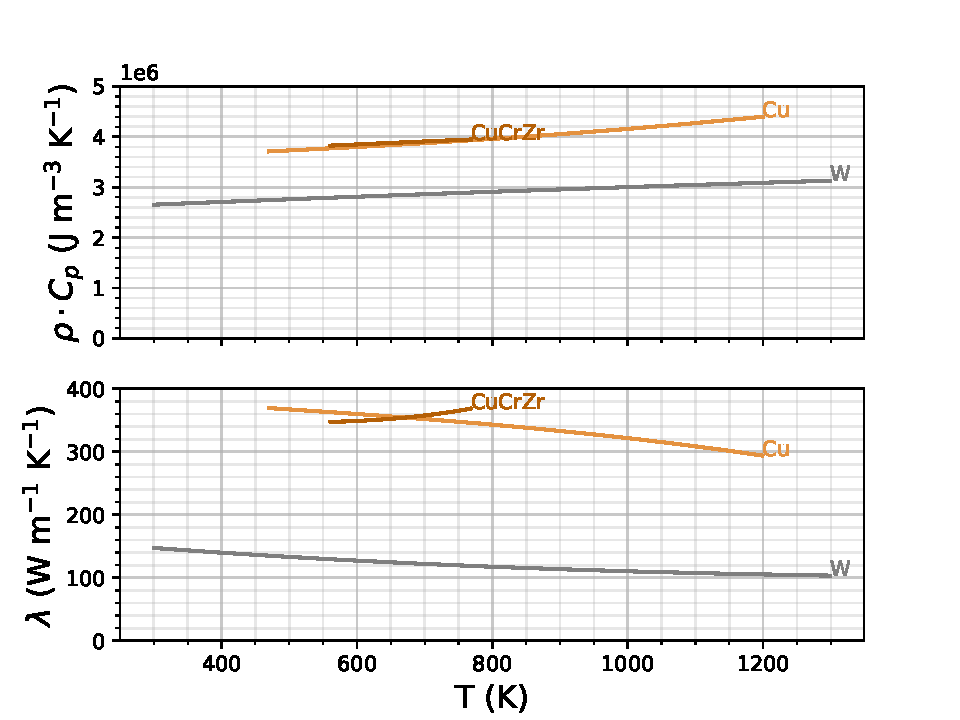
\includegraphics[width=\linewidth]{Figures/Chapter3/monoblocks/parametric_study/thermal_prop.pdf}
        \label{fig:thermal prop}
    \end{subfigure}%
    \begin{subfigure}{0.5\linewidth}
        \centering
        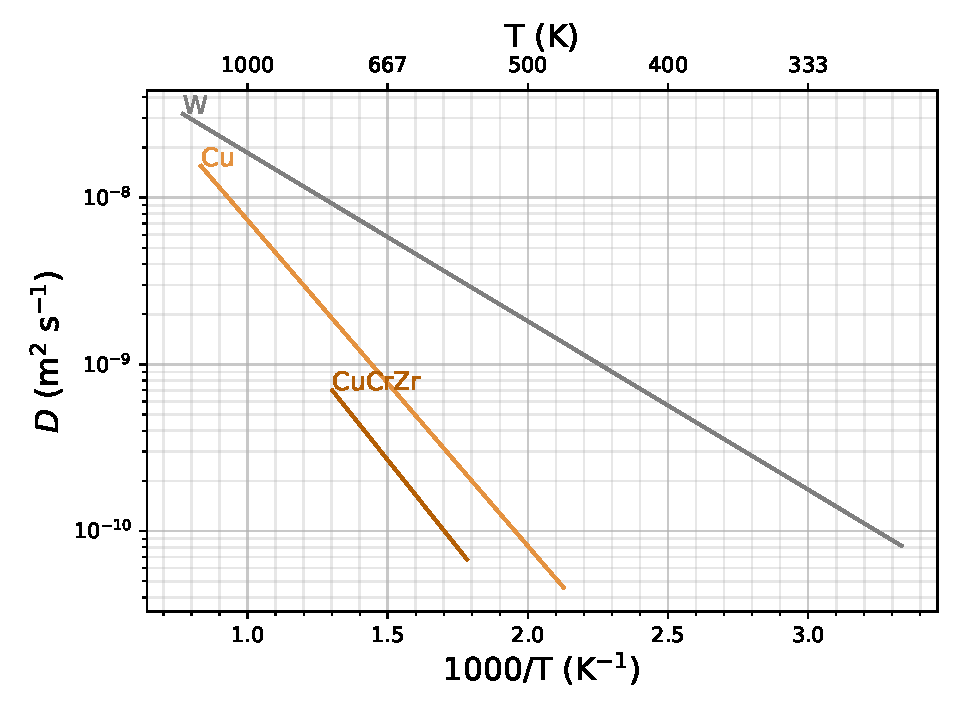
\includegraphics[width=\linewidth]{Figures/Chapter3/monoblocks/parametric_study/D_coeff.pdf}
        \label{fig:D coeff}
    \end{subfigure}
    \caption{Material properties used in the simulations \cite{reiter_compilation_1996, serra_hydrogen_1998, fernandez_hydrogen_2015}}
    \label{fig:properties}
\end{figure}

\begin{table*} [ht]
    \centering
    \begin{tabular}{L{1.5cm} L{1.5cm} R{1.6cm} R{1.1cm} R{1.6cm} R{1.1cm} R{2cm}}
         & Material & $k_0 (\si{m^3.s^{-1}})$ &  $E_k (\si{eV})$ & $p_0 (\si{s^{-1}})$ & $E_p (\si{eV})$ & $n_i (\si{at.fr.})$ \\
        \hline
        \\
       Trap 1 & W & $3.1 \times 10^{-16}$ & 0.20 & $8.4 \times 10^{12}$& 1.00 & $1.1 \times 10^{-3}$ \\
        \\
        Trap 2 & Cu & $6.0 \times 10^{-17}$ & \textcolor{black}{0.39} & $8.0 \times 10^{13}$ & 0.50 &$5.0 \times 10^{-5}$\\
        \\
        Trap 3 & CuCrZr & $1.2 \times 10^{-16}$ & \textcolor{black}{0.42} & $8.0 \times 10^{13}$ & 0.85 &$5.0 \times 10^{-5}$\\
        \\
    \end{tabular}
    \caption{Traps properties used in the simulations \cite{hodille_macroscopic_2015, dolan_assessment_1994}}
    \label{tab:traps monoblock}
\end{table*}

% \subsubsection{Boundary conditions}

Mobile particles concentration $c_\mathrm{m}$ is imposed on $\Gamma_\mathrm{top}$ which allows to simulate particle implantation without having to include a volumetric source term applied on the first few nanometres.
This approximation allows to have a broader mesh and therefore saves computation time without affecting the macroscopic behaviour.
Molecular recombination is assumed on $\Gamma_\mathrm{coolant}$.
Even though it could be assumed on the gaps between monoblocks, it can be shown that its influence on the macroscopic behaviour remains low.
Desorption from the other surfaces is therefore assumed to be zero for simplification purposes.
\textcolor{black}{Uniform} heat loads $\varphi_H$ are applied on the surface $\Gamma_\mathrm{top}$ with a Neumman boundary condition or temperature is constrained on $\Gamma_\mathrm{top}$ with a Dirichlet boundary condition and a convective exchange condition is set on surface $\Gamma_\mathrm{coolant}$.
All the other surfaces are assumed thermally insulated.
The set of boundary conditions can finally be described as follow:

\begin{eqnarray}
    -\lambda \vec{\nabla} T \cdot \vec{n} &=\varphi_{H} \quad \text{or} \quad T = T_\mathrm{surface}\quad &\text { on } \Gamma_\mathrm{top}\\
    \qquad \quad c_\mathrm{m} &=  c_\mathrm{surface}\quad &\text { on } \Gamma_\mathrm{top}\\
    -\lambda \vec{\nabla} T\cdot \vec{n} &= -h \cdot \left(T_\mathrm{coolant} - T\right)\quad &\text { on } \Gamma_\mathrm{coolant}\\
    -D \vec{\nabla} c_\mathrm{m} \cdot \vec{n} &= K_\mathrm{CuCrZr} \cdot c_\mathrm{m}^{2} \quad &\text { on } \Gamma_\mathrm{coolant}
\end{eqnarray}
with $h=\SI{70000}{W.m^{-2}.K^{-1}}$ being the heat exchange coefficient calculated from the Sieder-Tate correlation for the forced convection regime, $T_\mathrm{coolant}= \SI{323}{K}$ and $\vec{n}$ the normal vector and $K_\mathrm{CuCrZr} = 2.9 \times 10^{-14}\cdot \exp{(-1.92/(k_B\cdot T))}$ the recombination coefficient of the copper alloy (in vacuum) expressed in \si{m^4.s^{-1}} \cite{anderl_deuterium_1999}.

% The thermal response of ITER-like monoblocks to the heat load $\varphi_H$ has first been studied.
% Then the hydrogen inventory was determined as a function of surface temperature and surface concentration and as a function of the implanted particle flux and the incident ion energy.
% Finally, an application on ITER exposure conditions was made.

\subsection{Thermal behaviour}
Steady-state heat transfer simulations were performed with FESTIM with varying heat loads $\varphi_H$.
With $\varphi_H = \SI{1}{MW.m^{-2}}$, the surface temperature of the monoblock was found to be around \SI{400}{K} (see Figure \ref{fig:T field 1 MW}) whereas with $\varphi_H = \SI{10}{MW.m^{-2}}$ the surface was around \SI{1400}{K} (see Figure \ref{fig:T field 10 MW}).

\begin{figure*} [h!]
    \centering
    \begin{subfigure}{0.4\linewidth}
        \centering
        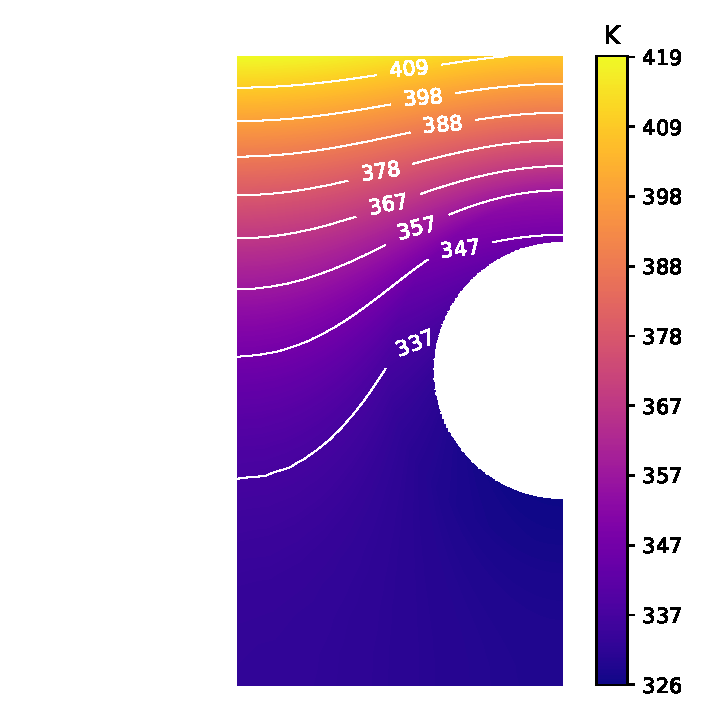
\includegraphics[width=\linewidth]{Figures/Chapter3/monoblocks/parametric_study/T_1e6.pdf}
        \caption{Temperature field with $\varphi_H = \SI{1}{MW.m^{-2}}$}
        \label{fig:T field 1 MW}
    \end{subfigure}%
    \begin{subfigure}{0.4\linewidth}
        \centering
        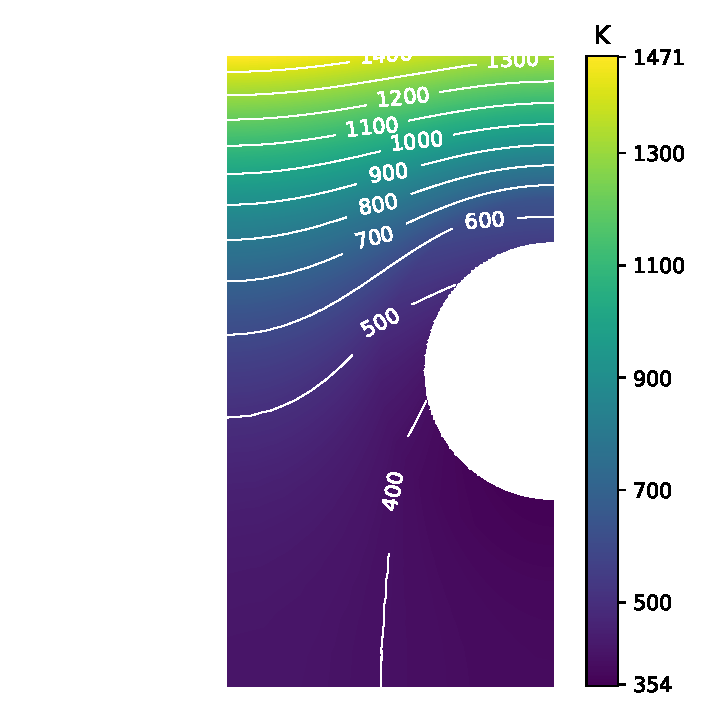
\includegraphics[width=\linewidth]{Figures/Chapter3/monoblocks/parametric_study/T_1e7.pdf}
        \caption{Temperature field with $\varphi_H = \SI{10}{MW.m^{-2}}$}
        \label{fig:T field 10 MW}
    \end{subfigure}
    \begin{subfigure}{0.7\linewidth}
        \centering
        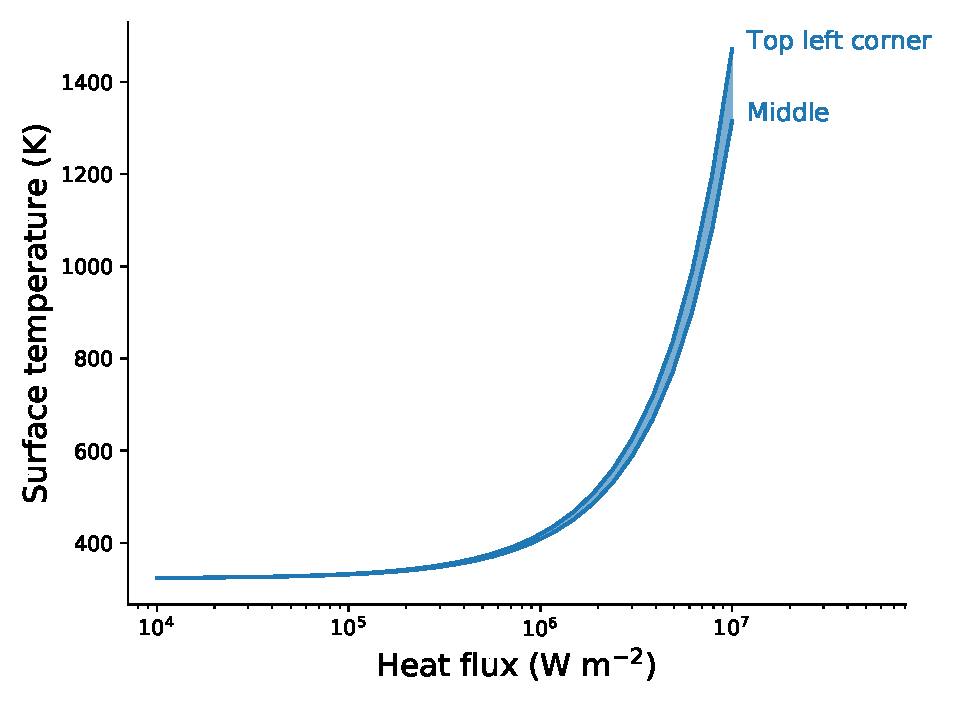
\includegraphics[width=\linewidth]{Figures/Chapter3/monoblocks/parametric_study/temperature_phi_H.pdf}
        \caption{\textcolor{black}{Evolution of surface temperature as a function of heat flux}}
        \label{fig:T phi_H}
    \end{subfigure}
    \caption{Thermal behaviour of the monoblock}
\end{figure*}

\textcolor{black}{
In order to simplify the analytical relations used in Section \ref{particle and energy}, only the mean surface temperature was considered in the following sections.
}
$T_\mathrm{surface}$ \textcolor{black}{therefore} increases linearly with the heat load and can be modelled by Equation \ref{eq:thermal behaviour law} (see Figure \ref{fig:T phi_H}).
\begin{equation}
    T_\mathrm{surface} = 1.1 \times 10^{-4} \cdot \varphi_H + T_\mathrm{coolant}
    \label{eq:thermal behaviour law}
\end{equation}

This was found to be in very good agreement with experimental measurements performed in \cite{hirai_use_2016}.

\subsection{Influence of \texorpdfstring{$T_\mathrm{surface}$}{Tsurface} and \texorpdfstring{$c_\mathrm{surface}$}{csurface} on hydrogen inventory}

In this section, the total inventory of hydrogen in monoblocks has been calculated as a function of $T_\mathrm{surface}$ and $c_\mathrm{surface}$.
Temperature and mobile concentration of hydrogen were imposed with Dirichlet boundary conditions on $\Gamma_\mathrm{top}$ with $T_\mathrm{surface}$ varying from $T_\mathrm{coolant}$ to \SI{1200}{K} and $c_\mathrm{surface}$ varying \textcolor{black}{arbitrarily} from \SI{e20}{m^{-3}} to \SI{6e22}{m^{-3}}.
The assumption of a constant surface temperature had low influence on the results compared to a non-homogeneous surface temperature that could be obtained with a heat flux condition since surface temperature gradient was low compared to the one between the top surface and the cooling surface.
For surface temperatures below \SI{500}{K}, 1D simulations were performed for the penetration depth of hydrogen remained very low (a few microns) and 1D approximation was sufficient \cite{benannoune_numerical_2019}.
For temperatures above \SI{500}{K} for which edge effects become dominant, 2D simulations have been performed.

After $ \SI{e7}{s}$ a high retention zone appeared far from the exposed surface $\Gamma_\mathrm{top}$ (see Figure \ref{fig:retention fields}).
As described in \cite{delaporte-mathurin_finite_2019}, this is due to thermal effects.
As seen in Figures \ref{fig:T field 1 MW} and \ref{fig:T field 10 MW}, the temperature was found to decrease in regions close to the cooling pipe $\Gamma_\mathrm{coolant}$ leading to an increase in trap occupancy, creating this high retention zone.
This was however not true for monoblocks where $T_\mathrm{surface} \approx T_\mathrm{coolant}$ since the temperature gradient in the domain is very low.
Instead, trap occupancy was close to one and the retention was high in the whole region where hydrogen had penetrated and not only far from the top surface.

\begin{figure*}
    \centering
    \begin{subfigure}{0.5\linewidth}
        \centering
        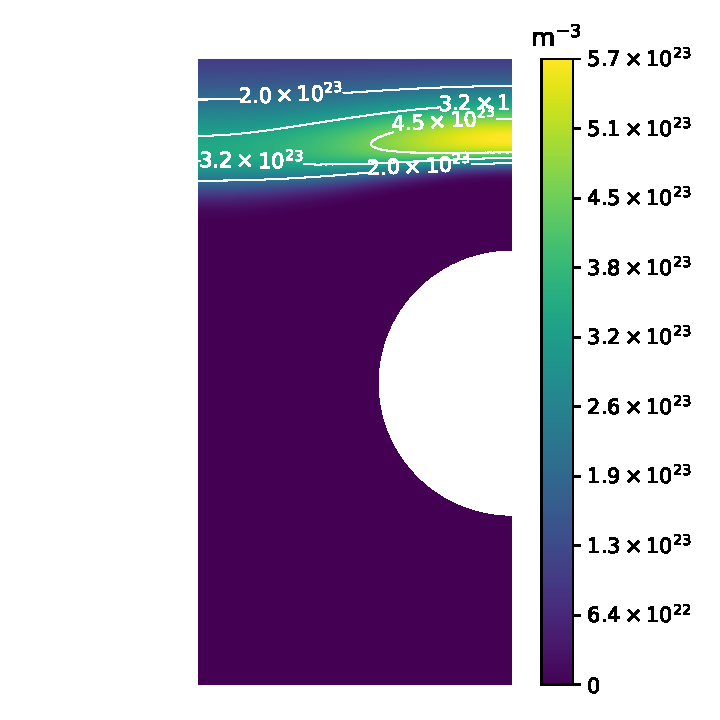
\includegraphics[height=\linewidth]{Figures/Chapter3/monoblocks/parametric_study/retention_T=7.000e+02;c=1.00e+20.pdf}
        \caption{$T_\mathrm{surface} = \SI{700}{K}$ and $c_\mathrm{surface} = \SI{e20}{m^{-3}}$}
    \end{subfigure}%
    \begin{subfigure}{0.5\linewidth}
        \centering
        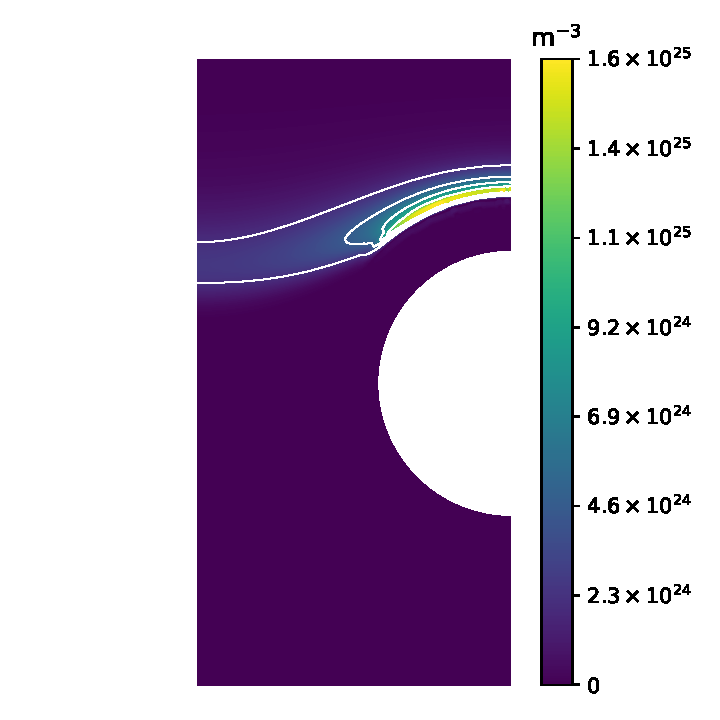
\includegraphics[height=\linewidth]{Figures/Chapter3/monoblocks/parametric_study/retention_T=1.000e+03;c=1.00e+21.pdf}
        \caption{$T_\mathrm{surface} = \SI{1000}{K}$ and $c_\mathrm{surface} = \SI{e21}{m^{-3}}$}
    \end{subfigure}
    \caption{Retention fields in \si{m^{-3}} after a \SI{e7}{s} exposure}
    \label{fig:retention fields}
\end{figure*}


Hydrogen inventory in monoblocks as a function of $T_\mathrm{surface}$ and $c_\mathrm{surface}$ is shown in Figure \ref{fig:inventory T c}.
In order to obtain this continuous field, more than 600 simulations randomly distributed on the parameter plane were run and analysed using a Gaussian process machine learning algorithm \cite{rasmussen_gaussian_2006} as in \cite{shimwell_multiphysics_2019} based on the python package inference-tools \cite{chris_bowman_c-bowmaninference-tools_2020}.
In Figure \ref{fig:inventory T c}, the inventory obtained by the Gaussian regression process is given for a constant value of $c_\mathrm{surf}=\SI{2e21}{m^{-3}}$ (top inset) and a constant temperature $T=\SI{850}{K}$ (left inset).
The Gaussian regression process was particularly appropriate as it calculates a confidence interval based on the standard deviation $\sigma$.
As expected, the lower the density of simulation points, the higher was the value of $\sigma$ (for example around \SI{850}{K} on the top inset of Figure \ref{fig:inventory T c}).
However, despite the lack of simulation in this region, the value of $\sigma$ was still acceptable (only a few percents of the inventory) ensuring the quality of the resulting interpolation.

As expected, inventory was found to globally increase with $c_\mathrm{surface}$.
For $T_\mathrm{surface} > \SI{550}{K}$, the inventory tended to decrease with surface temperature.
However, for $T_\mathrm{surface} < \SI{550}{K}$, inventory increased with surface temperature.
This phenomenon is due to a trade-off between an increase of the detrapping rate and an increase of the diffusion coefficient making the hydrogen particles penetrate deeper into the bulk.
Above $\SI{550}{K}$, detrapping becomes dominant and inventory decreases.
This mapping of inventory as a function of $T_\mathrm{surface}$ and $c_\mathrm{surface}$ provides an easy way of estimating the inventory in monoblocks for several exposure conditions without having to run many simulations.
Indeed, to estimate the inventory with different exposure conditions, one only needs to associate these conditions $(\varphi_\mathrm{inc}, E)$ to a couple $(c_\mathrm{surf}, T_\mathrm{surf})$.

\begin{figure*} [h]
    \centering
    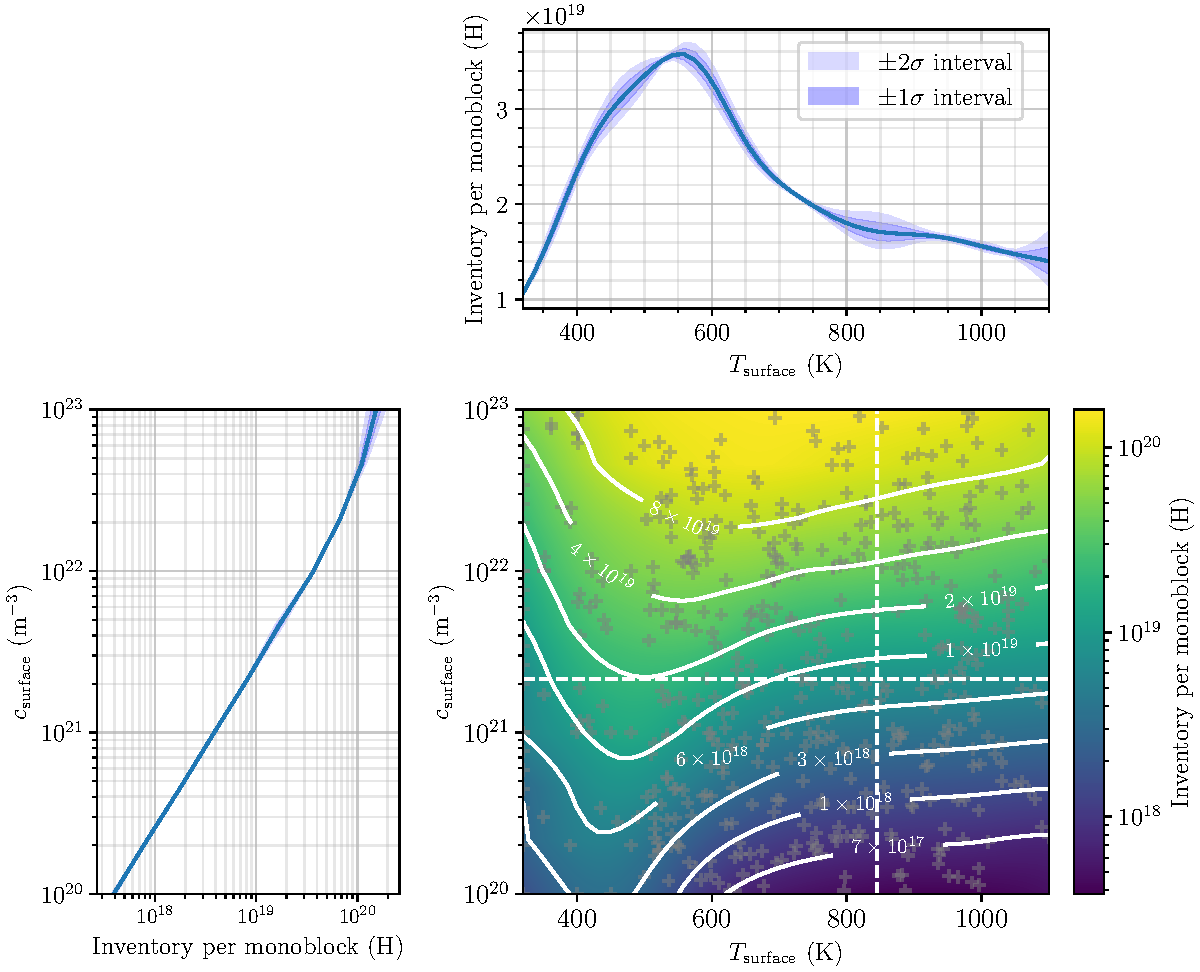
\includegraphics[width=\linewidth]{Figures/Chapter3/monoblocks/parametric_study/inventory_T_c_profiles.pdf}
    \caption{Evolution of the inventory after a \SI{e7}{s} exposure as a function of $T_\mathrm{surface}$ and $c_\mathrm{surface}$ alongside with simulation points (grey crosses). The simulations points were fitted with a Gaussian regression process \cite{chris_bowman_c-bowmaninference-tools_2020} providing the standard deviation $\sigma$.}
    \label{fig:inventory T c}
\end{figure*}

\subsection{Influence of incident particle flux and ion energy on hydrogen inventory} \label{particle and energy}
Incident particle flux $\varphi_\mathrm{inc}$ and ion energy $E$ have an impact on the amount of mobile particles implanted in the material but also on the heat load and therefore on the surface temperature of the monoblock.

Assuming a source term with a narrow Gaussian distribution and a non-instantaneous recombination (characterised by a recombination coefficient $K$), the concentration $c_\mathrm{max}$ at the near surface is approximated by:

\begin{equation}
    c_\mathrm{max} =  \frac{\varphi_\mathrm{imp} \cdot R_p}{D(T_\mathrm{surface})} + \sqrt{\frac{\varphi_\mathrm{imp}}{K(T_\mathrm{surface})}}
    \label{eq:cmax}
\end{equation}

where $\varphi_\mathrm{imp} = (1-r) \cdot \varphi_\mathrm{inc}$ is the implanted particle flux, $r$ is the particle reflection coefficient, $K$ is the recombination coefficient, and $R_p$ is the mean implantation depth in \si{m}.
Details can be found in appendix \textcolor{black}{as Supplementary Material}.
Many different values of the recombination coefficient $K$ for tungsten can be found in literature.
For instance the widely used Anderl coefficient describes an endothermic recombination \cite{anderl_hydrogen_1990} whereas Ogorodnikova showed an exothermic recombination coefficient could be used to reproduce a set of experiments \cite{ogorodnikova_recombination_2019}.

Facing the difficulty of an accurate choice for $K$ and following the recommendation of Causey \textit{et al} \cite{causey_hydrogen_2002}, an instantaneous recombination will therefore be assumed (\textit{ie} $K \rightarrow +\infty$).
It is also worth noting that experiments by Bisson \textit{et al} \cite{bisson_dynamic_2015} support the fact that recombination is not the rate limiting step during the hydrogen release from polycrystalline tungsten after ion implantation.

In the following, the concentration on $\Gamma_\mathrm{top}$ was set to $c_\mathrm{surface} = c_{\mathrm{max}}$ for the kinetics involved are really fast (see appendix of \cite{hodille_hydrogen_2018}) and $R_p$ is small compared to the monoblock dimensions.

The heat load was assumed to evolve as a function of the incident particle flux $\varphi_\mathrm{inc}$ and $E$ as follow:

\begin{equation}
    \varphi_H = 2.2\cdot \varphi_\mathrm{inc} \cdot e \cdot (E + \SI{13.6}{eV})
    \label{eq:phi_H}
\end{equation}
with $e = \SI{1.6e-19}{C}$.
This relation was obtained by fitting SOLPS \textcolor{black}{data \cite{pacher_impurity_2015, khan_walldyn_2019}}.
The factor 2.2 was applied to take into account other heat sources such as radiative flux.

Moreover, the ion energy $E$ has an influence on $r$ and implantation range $R_p$ and it was possible to model the evolution of these parameters with SRIM \cite{ziegler_srim_2010} calculations as follow:
\begin{equation}
    r = 2\times 10^{-8} \cdot E^2 -6 \times 10^{-5} \cdot E + 8\times 10^{-1}
    \label{eq:r}
\end{equation}

\begin{equation}
    R_p = 1.4\times 10 ^{-10}\cdot E^{0.64}
    \label{eq:Rp}
\end{equation}
By combining Equations \ref{eq:phi_H}, \ref{eq:r}, one can obtain the evolution of $\varphi_H$ as a function of $\varphi_\mathrm{inc}$ and $E$ as shown in Figure \ref{fig:phi_H phi E}.
From the thermal behaviour given by Equation \ref{eq:thermal behaviour law}, the surface temperature $T_\mathrm{surface}$ can be computed (see Figure \ref{fig:T_surf phi E}).
Finally, $c_\mathrm{max}$ was obtained from Equations \ref{eq:cmax} and \ref{eq:Rp} (see Figure \ref{fig:c_max_instantaneous}).

\begin{figure*} [ht]
    \centering
    \begin{subfigure}{0.5\linewidth}
        \centering
        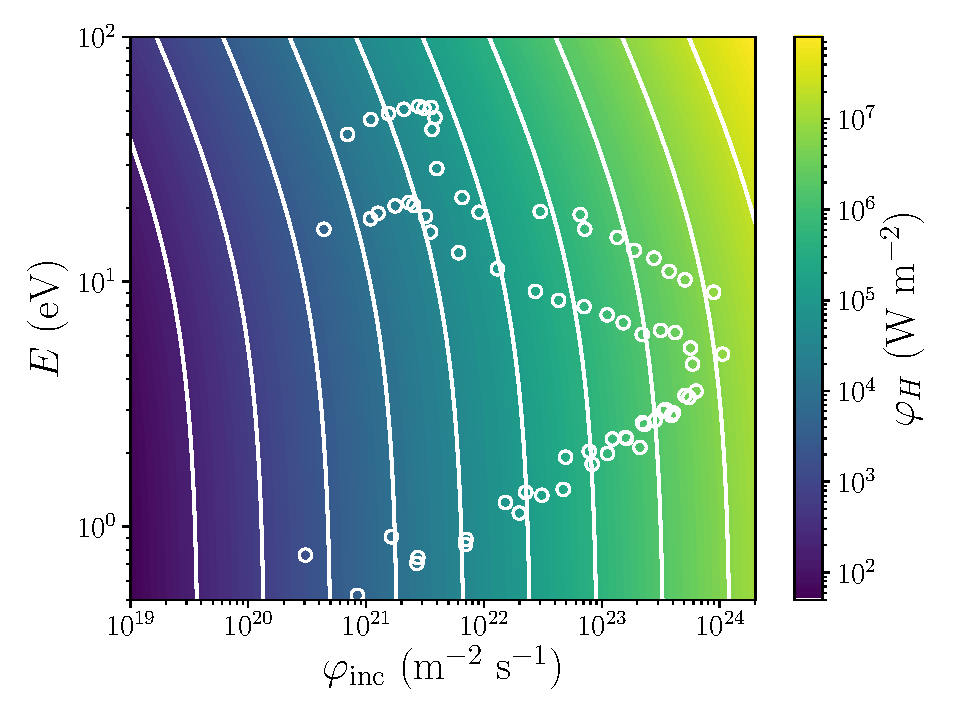
\includegraphics[width=\linewidth]{Figures/Chapter3/monoblocks/parametric_study/phi_H_phi_E.pdf}
        \caption{Surface heat flux}
        \label{fig:phi_H phi E}
    \end{subfigure}%
    \begin{subfigure}{0.5\linewidth}
        \centering
        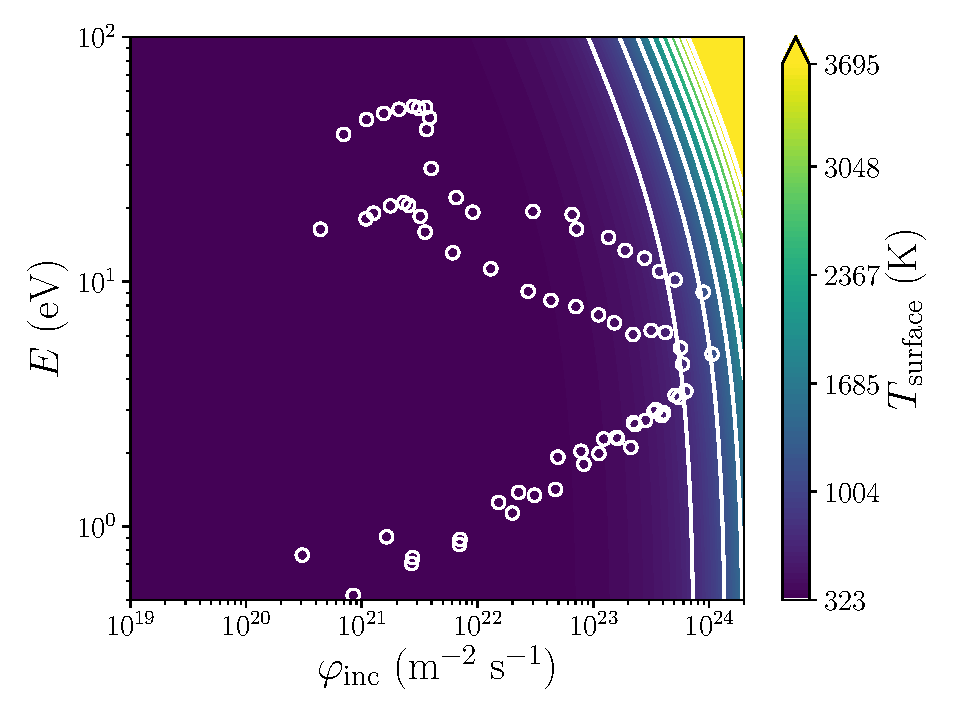
\includegraphics[width=\linewidth]{Figures/Chapter3/monoblocks/parametric_study/T_phi_E.pdf}
        \caption{Surface temperature}
        \label{fig:T_surf phi E}
    \end{subfigure}
    \begin{subfigure}{0.5\linewidth}
        \centering
        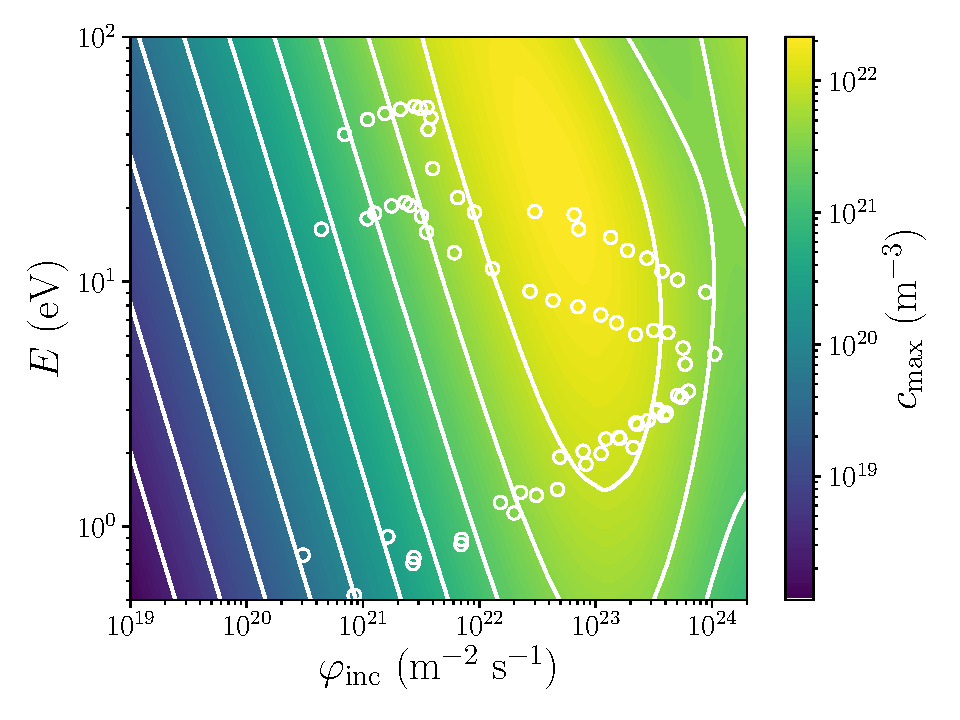
\includegraphics[width=\linewidth]{Figures/Chapter3/monoblocks/parametric_study/c_max_instantaneous.pdf}
        \caption{Surface concentration}
        \label{fig:c_max_instantaneous}
    \end{subfigure}%
    \begin{subfigure}{0.5\linewidth}
        \centering
        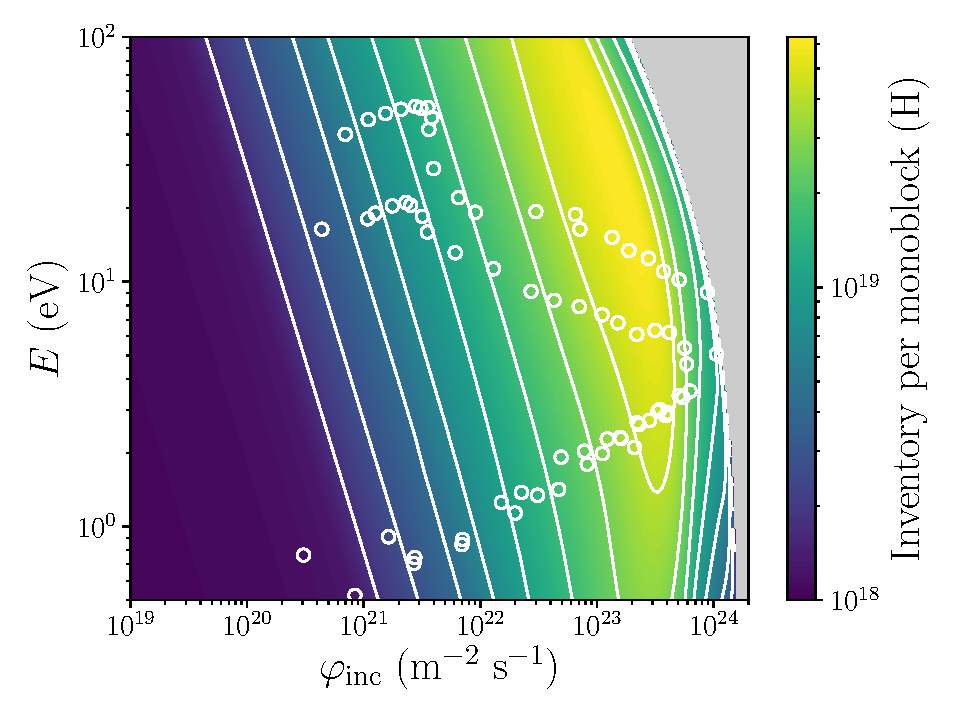
\includegraphics[width=\linewidth]{Figures/Chapter3/monoblocks/parametric_study/inventory_phi_E.pdf}
        \caption{Monoblock inventory}
        \label{fig:inventory phi E}
    \end{subfigure}
    \caption{$\varphi_H$, $T_\text{surface}$, $c_\mathrm{max}$ and inventory per monoblock as a function of $\varphi_\mathrm{inc}$ and $E$. Inventory has not been calculated for surface temperature above \SI{1200}{K} (greyed region). White circles correspond to points on ITER divertor using the divertor plasma parameters from SOLPS \cite{bonnin_presentation_2016} calculations (see Section \ref{ITER application}).}
    \label{fig:phi_H T_surf c_max}
\end{figure*}

One must be aware that above \SI{1500}{K}, W recrystallisation can occur and H transport will strongly be affected.
The hypothesis made above as well as material properties may then not be valid.
Because of the trade-off between the amount of implanted particles and the resulting heat flux, the maximum value of $c_{\mathrm{max}}$ was found to be \SI{2e22}{m^{-3}} around $(\varphi_\mathrm{inc}, E)=(\SI{8e22}{m^{-2}.s^{-1}}, \SI{20}{eV})$.
Considering the previously calculated response of the monoblock to $c_\mathrm{surface}$ and $T_\mathrm{surface}$ (see Figure \ref{fig:inventory T c}), the inventory as a function of $\varphi_\mathrm{inc}$ and $E$ was computed (see Figure \ref{fig:inventory phi E}).
The inventory values have not been calculated for surface temperatures above \SI{1200}{K}.
Again a trade-off was found between implanted particle flux and surface temperature.
Indeed, the maximum inventory was not found at regions where the incident flux is maximum but rather at regions where $c_\mathrm{surface}$ is maximum and $T_\mathrm{surface}$ is minimum as seen in previous 1D studies \cite{hodille_estimation_2017}.

\subsection{Application to tokamak exposure conditions} \label{ITER application}
Each white circle in Figure \ref{fig:phi_H T_surf c_max} corresponds to a point along a poloidal section of the ITER divertor for which implanted particle flux and ion energy were calculated with SOLPS \cite{bonnin_presentation_2016} for a partially detached plasma scenario.
This scenario corresponds to a $Q=10$ discharge with a neutral pressure of \SI{8.6}{Pa} \cite{pitts_physics_2019}.


\begin{figure*} [t]
    \centering
    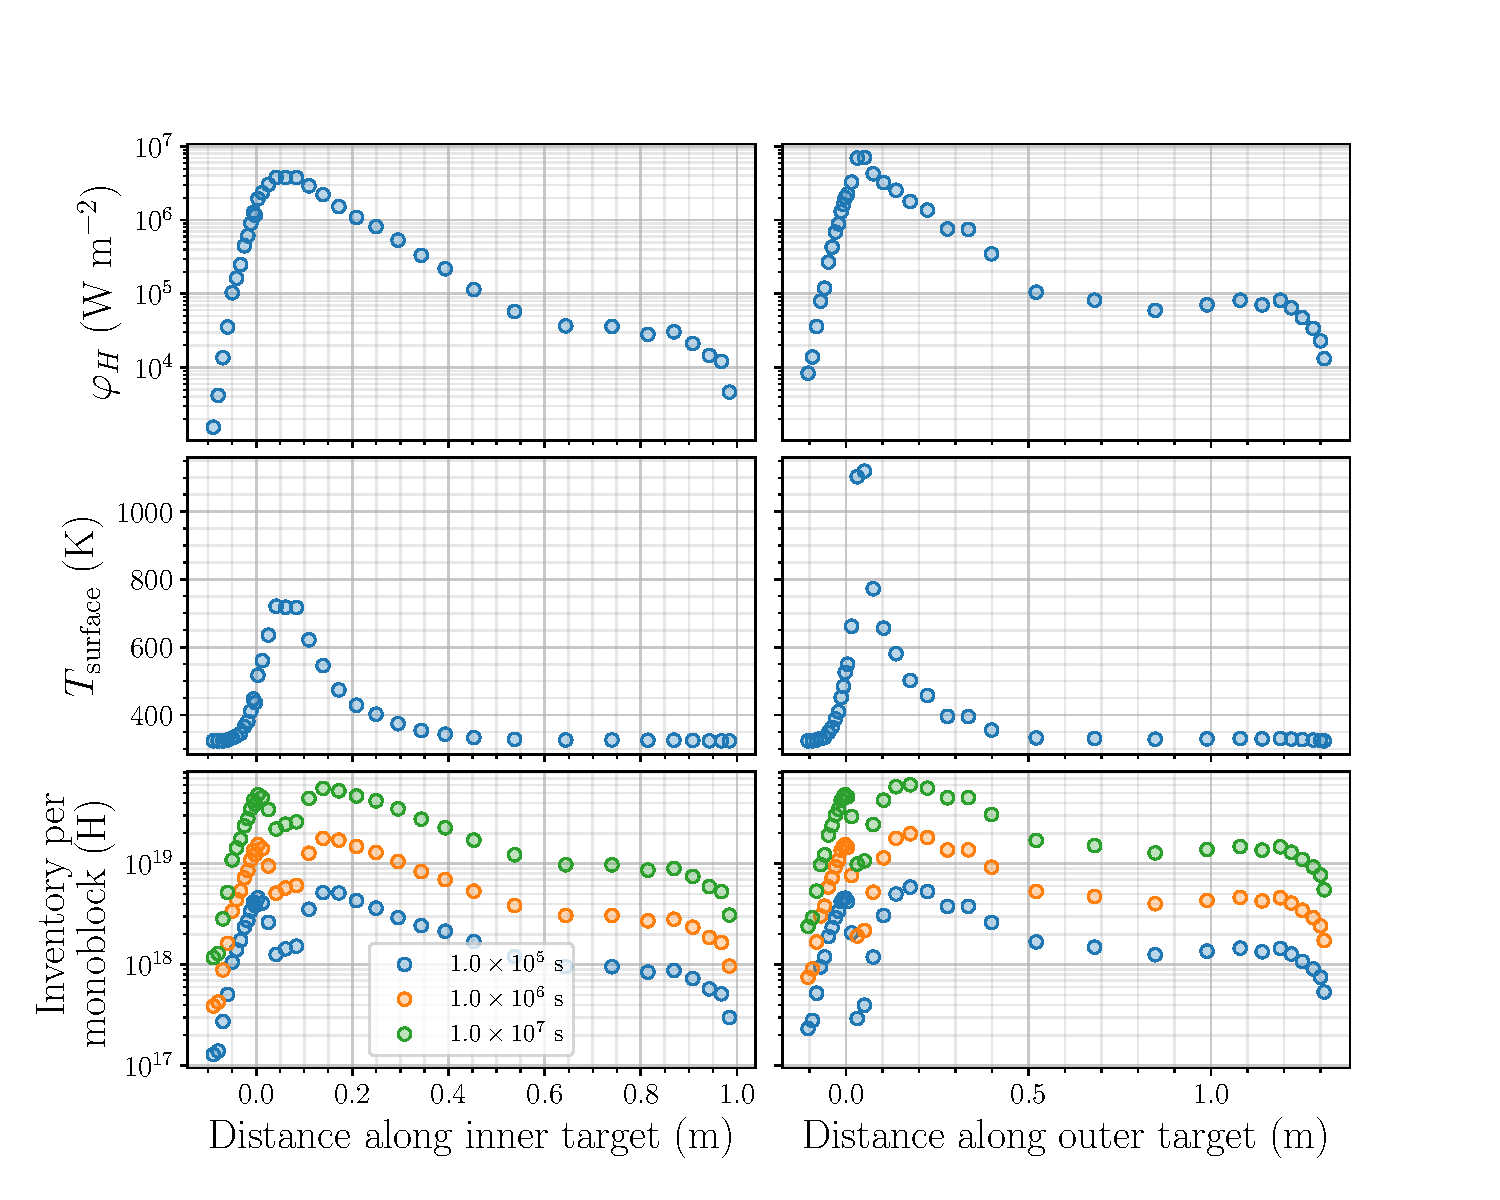
\includegraphics[width=0.8\linewidth]{Figures/Chapter3/monoblocks/parametric_study/along_divertor.pdf}
    \caption{Evolution of $\varphi_H$ (top), $T_\mathrm{surface}$ (middle) and inventory (bottom) after several exposure times along a poloidal section of the divertor for inner vertical target and outer vertical target.}
    \label{fig:along divertor}
\end{figure*}

As expected the highest surface temperatures and heat loads were located on strike points and most of the zones on the divertor were found to stay at coolant temperature (see Figure \ref{fig:along divertor}).
The maximum hydrogen content is approximately \SI{6e19}{H} per monoblock after a \SI{e7}{s} exposure.
As explained in the previous section, the maximum inventory is not necessarily in the region where the flux is maximum as it induces a higher temperature which will tend to increase detrapping: strike points are not where hydrogen is trapped the most.
Instead, the maximum inventory is reached about \SI{5}{cm} away from the strike points where the temperature and the fluxes are high enough to guarantee a strong source of mobile particle but the temperature is not high enough to trigger detrapping.

For all points on the divertor, the inventory evolved as $a \cdot t^b$ as shown in Figure \ref{fig:inv_vs_time} for particular points on the inner vertical target ($x=0.03$ m is close to the strike point).
The coefficient $b$ is maximum on strike points reaching 0.75 (see Figure \ref{fig:a_b_along_div}).
In other regions, $b$ is closer to 0.5.
This result can be explained by the non-homogeneous temperature field in monoblocks with high heat loads.
For monoblocks with a high surface temperature, as hydrogen penetrates deeper into the bulk, the bulk temperature decreases (see Figure \ref{fig:T field 10 MW}) leading to an increase of the trap occupancy \cite{hodille_estimation_2017}.
The exponent $b$ is therefore higher than $0.5$.
For monoblock where $T_\mathrm{surface} \approx T_\mathrm{coolant}$ on the other hand, the temperature is homogeneous in the whole domain and $b=0.5$.
This corresponds to a diffusion-limited behaviour.

The temperature is close to $T_\mathrm{coolant}$ and the trap occupancy is therefore close to one in the whole domain which is not the case for regions near strike points where temperature fields are non-uniform.

\begin{figure} [t]
    \centering
    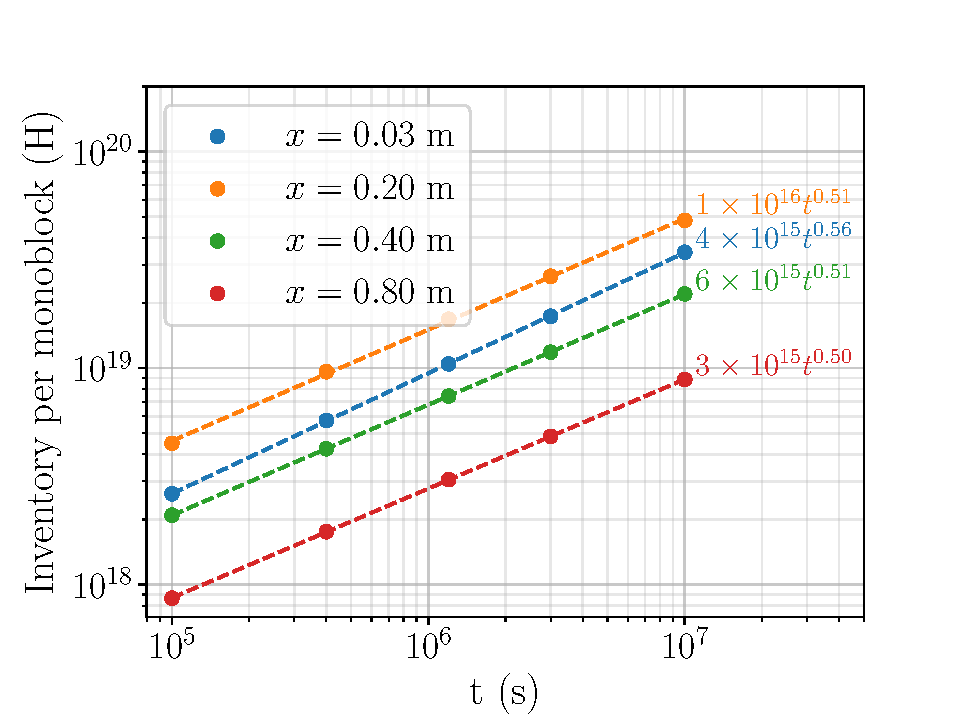
\includegraphics[width=0.5\linewidth]{Figures/Chapter3/monoblocks/parametric_study/inventory_vs_time.pdf}
    \caption{Temporal evolution of hydrogen inventory in monoblocks at several locations on inner vertical target of ITER divertor}
    \label{fig:inv_vs_time}
\end{figure}


\begin{figure*} [h]
    \centering
    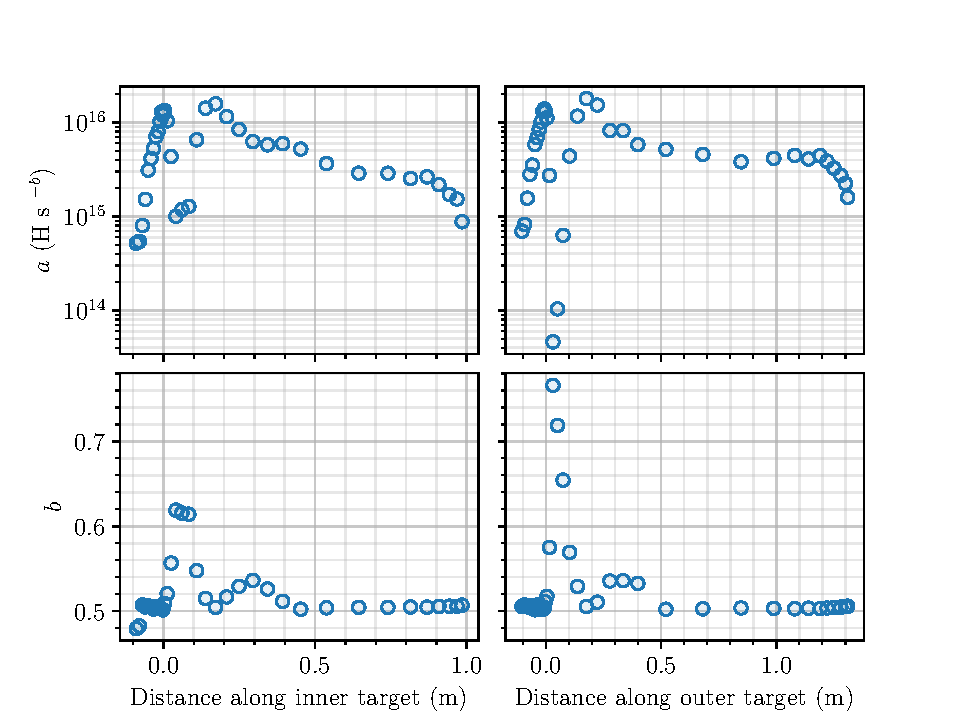
\includegraphics[width=0.8\linewidth]{Figures/Chapter3/monoblocks/parametric_study/a_b_along_div.pdf}
    \caption{Evolution of coefficients $a$ and $b$ along a poloidal section of the divertor. Inventory evolves as $a\cdot t^b$ (H).}
    \label{fig:a_b_along_div}
\end{figure*}

One can obtain the inventory in the whole divertor by integrating the results obtained in Figure \ref{fig:along divertor} over the tokamak as follow:

\begin{eqnarray}
    \mathrm{inv_{divertor}} = N_\mathrm{cassettes}
    \cdot \left(N_\mathrm{PFU-IVT} \cdot \int \mathrm{inv_{IVT}}(x)\: dx + N_\mathrm{PFU-OVT} \cdot\int \mathrm{inv_{OVT}}(x) \: dx \right)
\end{eqnarray}
with $N_\mathrm{cassettes}=54$ the number of cassettes, $N_\mathrm{PFU-IVT}=16$ and $N_\mathrm{PFU-OVT}=22$ the number of plasma facing units per cassette on the inner and outer targets respectively, $\mathrm{inv_{IVT}}$ and $\mathrm{inv_{OVT}}$ the hydrogen inventory profile along the inner and outer targets respectively and $x$ the distance along the targets.

\begin{figure} [h]
    \centering
    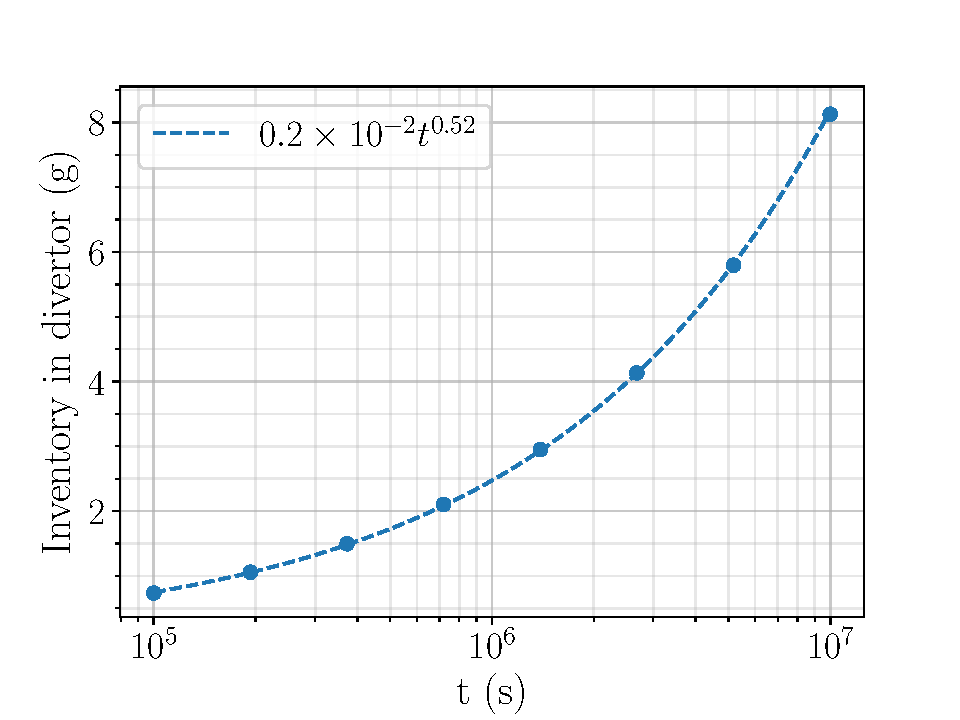
\includegraphics[width=0.5\linewidth]{Figures/Chapter3/monoblocks/parametric_study/inventory_divertor.pdf}
    \caption{Temporal evolution of hydrogen inventory in the whole divertor}
    \label{fig:inventory divertor}
\end{figure}

After a \SI{e7}{s} exposure, hydrogen inventory is estimated at approximately \SI{8}{g} (see Figure \ref{fig:inventory divertor}) which is relatively low considering the ITER in-vessel limit and the elapsed time.
De Temmerman \textit{et al} showed that retention in ITER can reach \SI{0.3}{g} per \SI{400}{s} discharge when taking into account Be deposits.


\subsection{Discussion}
If this methodology provides a rapid way of estimating hydrogen content in the whole divertor, several assumptions have however been made.


% Influence of cycling
First, a steady state exposure was considered for simplification purposes.
This result is however conservative.
As seen in \cite{delaporte-mathurin_finite_2019, hodille_estimation_2017}, cycling effects could have an influence in regions where $T_\mathrm{surface}$ varies a lot, for example \textcolor{black}{within \SI{10}{cm} on both sides of the strike points}.
Though, since a large majority of monoblocks were found to stay at room temperature, even during operations (see Figures \ref{fig:T_surf phi E} and \ref{fig:along divertor}) the thermal effect should remain low and discrepancies would rather be due to particle flux evolution along the target.

% shaping
\textcolor{black}{
Shaping of monoblocks (\textit{e.g.} chamfers) was not taken into account in this work for simplification purposes.
Such shaping can have an influence on the incident particle and heat loads on the plasma facing surface of the monoblocks.
}


% Be deposits
This study presents the hydrogen trapping in W monoblocks.
It shows that the latter remains low but, as already pointed out by JET studies, the trapping on Be co-deposited layers is expected to be the main mechanism for tritium retention in ITER \cite{brezinsek_beryllium_2015, heinola_fuel_2015}.
Such layers could be found in the cold regions of the divertor but as soon as the strike points hit these layers, they should be sputtered away (as sputtering of Be is possible even at low energy \cite{bjorkas_variables_2013, brezinsek_beryllium_2015}).
The retention where the deposited layers are not present (either sputtered or not formed anyway) would then be given by the model presented here.

% Coolant recombination
\textcolor{black}{
The molecular recombination coefficient at the surface of the cooling pipe was taken from \cite{anderl_deuterium_1999} and was measured in vacuum.
One could argue that recombination in presence of water will be facilitated.
It can however be shown that this parameter has very low influence on the inventory since it was dominated by retention in tungsten.
This parameter will however have an influence on the permeation flux and should be studied in future work.}

% Gap recombination
\textcolor{black}{Similarly, the influence on molecular recombination on the sides of the monoblock was found to have a low impact on the results.
By assuming an instantaneous recombination coefficient, the relative error on the monoblock inventory was found to be significant only in hot regions (\textit{ie} within \SI{10}{cm} on both sides of the strike points).
The influence on the total divertor inventory is therefore low (less than \SI{5}{\%} after a \SI{e7}{s} exposure) since it is dominated by regions where $T_\mathrm{surface} \approx T_\mathrm{coolant}$.}

% ELMs
It should be noted that specific scenarii like edge localised modes (ELMs) were also not taken into account in this work since their time scale is very short.
MRE simulations by Hu and Hassanein \cite{hu_predicting_2015} suggest that a \SI{400}{s} discharge with \SI{1}{Hz} or \SI{10}{Hz} ELMs significantly reduces (77 \%) the inventory in W materials.
However, the modelling of the ELM is simulated by increasing the temperature for a very short time without changing the incident flux of particles that can also be much higher thus balancing the fuel retention reduction.
Another study by Schmid \textit{et al} \cite{schmid_diffusion-trapping_2016} also simulated the effect of \SI{1}{Hz} ELMs on fuel retention in W.
The outcome is that \SI{6}{s} of \SI{1}{Hz}-ELMs does not affect significantly the fuel retention, though the temperature excursion in those simulations are smaller than for the one of Hu and Hassanein.
Thus, the effect of ELMs, especially the balance between increase of heat flux, incident energy and particle flux, could either favour or disfavour trapping, diffusion and migration and therefore the overall retention.

% Surface process
In this study the model to link the concentration of mobile particles at the surface (implantation zone) with the exposure condition considers that the particles are implanted in the bulk and that the recombination coefficient is very high since many uncertainties concerning the recombination coefficient are yet to be lifted.
However, if an exothermic process is considered as in \cite{ogorodnikova_recombination_2019}, this should have low influence since recombination is very quick at a temperature close to that of the coolant.

On the other hand, experimental results \cite{t_hoen_strongly_2013} suggest that for ion energy below \SI{5}{eV/H}, typical of detached plasma as the one treated in the previous section, the surface process can be important and limits the uptake of hydrogen, i.e. the adsorption on the surface and the further absorption from surface to bulk could be the limiting process for the growth of $c_\mathrm{surface}$ during such exposure.
The evolution of $c_\mathrm{surface}$ to the exposure condition for that range of energy would therefore be different and therefore the inventory.
The advantage of the presented method is that taking into account such process is realtively easy as no expensive simulations are needed.
One would only need to modify the model giving $c_\mathrm{surface}$
as a function of $(E_\mathrm{inc},\varphi_\mathrm{inc})$ to include the different surface processes.
To this end, one can use kinetic surface models \cite{hodille_retention_2017, zaloznik_deuterium_2017, pecovnik_influence_2019, guterl_effects_2019}.

% traps
\textcolor{black}{
Trap properties have a great impact on the inventory.
In this study, a homogeneous trap distribution is assumed for simplification purposes.
A more thorough study could investigate the influence on trap distribution, energy and density.
Trap properties might also vary along the divertor based on exposure conditions.
Moreover the impact of neutrons must be assessed as neutron-induced traps have a high detrapping energy.
}

% Helium
\textcolor{black}{
Finally, helium implantation in the materials and bubble formation could modify the hydrogen transport in monoblocks.
}